\documentclass[]{article}
% packages
\usepackage{../../cs70}
\usepackage{../../markup}
\usepackage{enumerate}
\usepackage{hyperref}
%% \usepackage{framed}
%% \usepackage{MnSymbol}
%% \usepackage{epstopdf}
\usepackage{color}
%% \usepackage[]{amsmath}
%% \usepackage{graphicx}
%% \usepackage{amssymb}
%% \usepackage{parskip}
%% \usepackage{rotating}
%% \usepackage{float}
%% \usepackage{multirow}
%% \usepackage{subcaption}
%% \usepackage{indentfirst}
%% \usepackage[left=1.5in, right=1.0in, top=1.0in, bottom=1.0in]{geometry}

\newif\ifsolutions
\newif\ifmotivation
\motivationtrue
\motivationfalse
\solutionstrue
%\solutionsfalse %flag for solutions

\renewcommand{\answer}[1]{{\color{mydarkblue}\textbf{Solution:}#1}}
\definecolor{mydarkblue}{rgb}{0,0.25,1}

\def\title{Homework 9}

\begin{document}

\maketitle
\config{hwnum}{9}
\config{homework-due}{03/31/2014 13:00}
\config{grades-due}{04/07/2014 13:00}
\vspace{0.5em}
{\Large{\textbf{This homework is due Mar 31 2014, at 12:00 noon.}}}

\begin{qunlist}
  
\qns{Virtual Lab 3: Biased Coins Continued}\\    
In this problem we will continue the lab from last HW. We will start from the optional problem at the end.
\begin{enumerate}[a)]


\qpart 
\item  Up till this point, everything that
  you have done in this virtual lab is something that you could've
  naturally discovered yourself as something worth trying. The data is
  speaking directly to the experimentalist in you. However,
  discovering an actual formula for the shape of this ``cliff-face'' is
  something that actually requires a theoretical investigation that is
  related to counting, Fourier Transforms, and Power Series. Guessing
  its exact shape is not something that comes very naturally on
  experimentalist intuition alone.

  So here, we will simply provide you with the right curve.

  Plot $\int_{-\infty}^d\frac{1}{\sqrt{2\pi}} e^{-\frac{x^2}{2}}dx$
  overlaid with the normalized cliff-face shapes you had plotted in
  the earlier parts. (Do this integral numerically or use the special
  functions that most numerical packages already have for computing
  these sorts of integrals. This integral is related to something
  called the Error Function.) Notice how beautifully it hits the exact
  shape. 

  This is the heart of the Central Limit Theorem as applied to coin
  tosses.

\ifsolutions{ \answer {
We can see that the theoretical curve fits the shape perfectly for different $p$ values. And the zigzags smooth out as $k$ increases.
\begin{figure}[h!]
\center
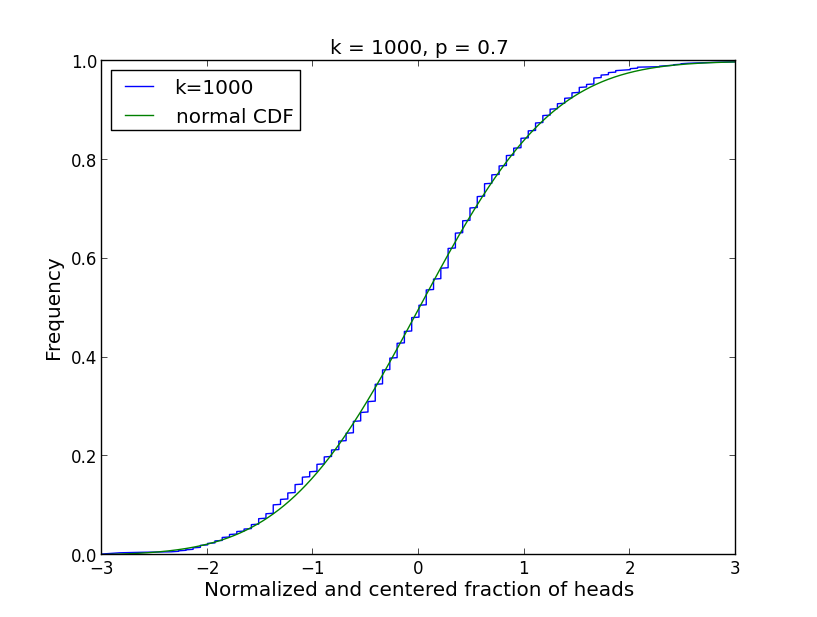
\includegraphics[width=0.9\textwidth]{figures/part_a.png}
\end{figure}

}}\fi


\newpage
 
\qpart
\item Just a little notation. We will use $X_i$ to denote a random
  variable that is 1 if you toss a head on the $i$-th toss, and 0 if you toss a
  tail on the $i$-th toss. (This is just so we can more easily express 
  things) So a sequence of $k$ coin tosses would be $X_1, X_2, \ldots,
  X_{k-1}, X_k$, with each $X_i$ being 0 or 1 depending on how the run
  actually came out. How would you write the total number $S$ of heads
  as a function of the $X_i$'s? 

 Our experience from the last homework tells us that the total number
 of heads is itself a random quantity since it varies based on the
 vagaries of the coin tosses.

\ifsolutions{ \answer { We can write $S_k$ as
\[ S_k = \sum_{i=1}^k X_i. \]
where the subscript $k$ denotes the number of coin flips.
}}\fi



\qpart 
\item Now, since you had realized earlier that the cliff-faces and the
  histograms have some natural relationship with each other, see if
  you can figure out a way to naturally overlay a smooth plot of
  $\frac{1}{\sqrt{2\pi}} e^{-\frac{x^2}{2}}$ to the normalized
  histograms. What does this mean?

\ifsolutions{ \answer { By normalizing the histograms by area so that the sum of the heights of all the bars equals 1, we can overlay the function above very nicely. This suggests that integrating these histograms will yield the cliff-face shapes plotted in part (a). It also suggests that the probability of getting certain numbers of heads is related to the normal distribution.

\begin{figure}[h!]
\center
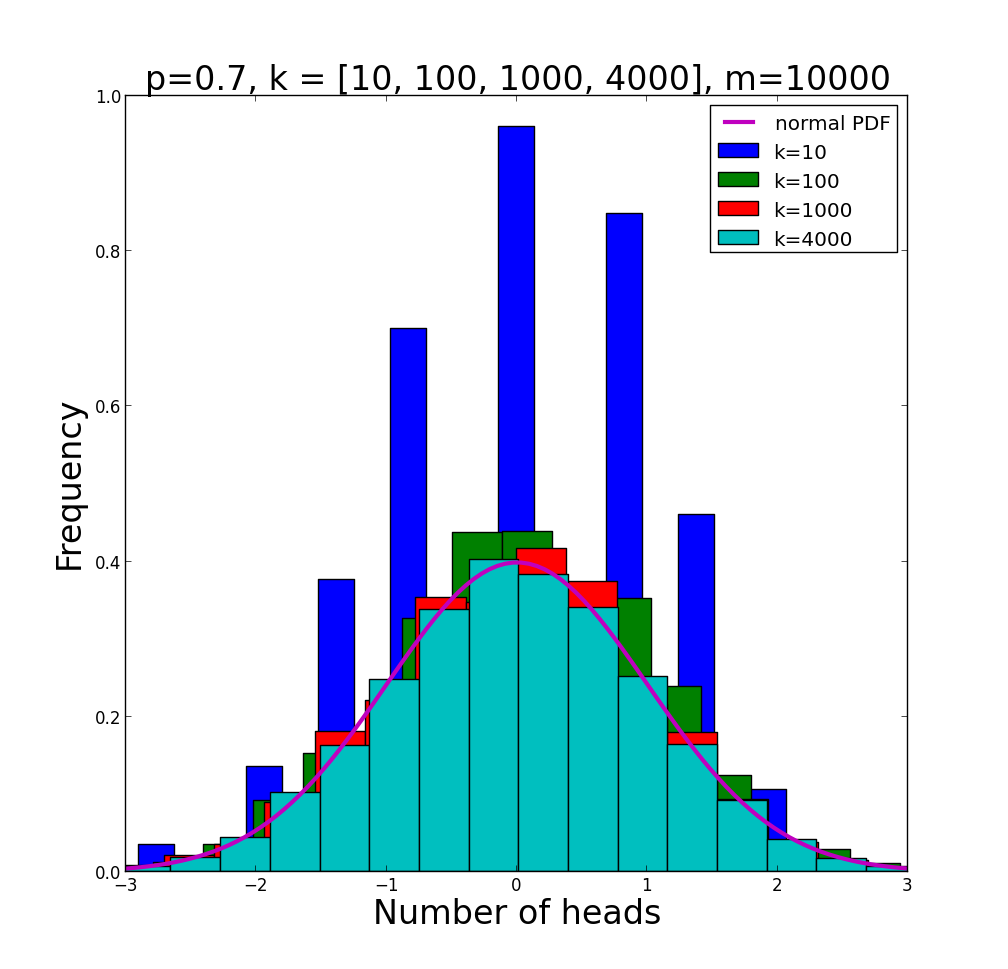
\includegraphics[width=0.9\textwidth]{figures/part_c.png}
\end{figure}
}}\fi


\newpage

\qpart
\item The other interesting pattern that you had seen in the previous
  virtual lab (In particular, in part k of Q1 on HW7) was the
  exponential drop in the frequencies of certain rare events. For an
  exponential drop, the most interesting thing is to understand the
  rate of the exponential --- or the relevant slope on the Log-Linear
  plot.  

  For a coin with probability $p$ of being heads, we are interested in
  the frequency by which tossing $k$ such coins results in more than
  $ak$ heads (where $a$ is a number larger than $p$). We are
  interested in $p=0.3,0.7$ and $a = p+0.05$,
  $p+0.1$.  Take $m = 10000$ and plot the natural log of the frequencies 
  these deviations against $k$ (ranging from 10 to 200). Approximately
  extract the slopes for all 4 of these.

  Compare them in a table against the predictions of the following
  formula (which we will derive later in the course)
  $$D(a||p) = a \ln \frac{a}{p} + (1-a) \ln \frac{1-a}{1-p}.$$
  
  This expression is called the Kullback-Liebler divergence and is also
  called the relative entropy. 

  Finally, add $e^{-D(a||p) k}$ to the plots (there should be 4 of
  these) you have made as straight lines for immediate visual
  comparison. This straight line is called a ``Chernoff Bound'' on the
  probability in question. 

  Comment. 

\ifsolutions{ \answer { After fitting lines to the Log-Linear plots below, we obtain the following table

\begin{table}[h!]
\center
\color{mydarkblue}{
\begin{tabular}{llcc}
$p$ & $a$ & fitted slope & $D(a||p)$ \\
\hline
0.3 & 0.35 & -0.00864 & 0.00578 \\
0.3 & 0.4 & -0.02686 & 0.02258 \\
0.7 & 0.75 & -0.00918 & 0.00616 \\
0.7 & 0.8 & -0.03090 & 0.02573 \\
\end{tabular}
}
\end{table}

We can see that the slope of the fitted lines are very close to the negative K-L divergence. Also, the table values for $a=p+0.05$ are quite similar, and the values for $a=p+0.1$ are also similar. In the log-linear plot, we can see that the function $e^{-D(a||p) k}$ runs parallel to the fitted lines for each ($p$,$a$) pair.


Suggestions for coding: $m=10,000$ takes a long time to run.  Take a lower $m$ at first for faster debugging. To fit a line, you can use "polyfit(x,y,1)" for linear fitting.  There will probably be some 0 values, which will mess up this fitting, so you can replace 0 values with $10^-3$ or something like that. Larger $m$ will probably elminate all the 0's.

\begin{figure}[h!]
\center
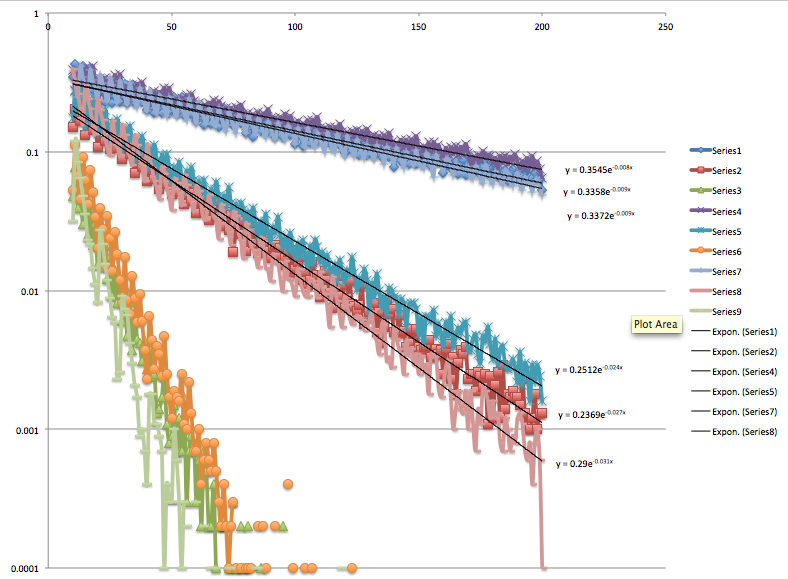
\includegraphics[width=0.9\textwidth]{figures/part_d.png}
\end{figure}
}}\fi


\newpage

\qpart
\item In the previous part, we went directly to one of the most
  powerful bounds we have. A much simpler bound (that we will
  rigorously derive later in the course) is called Chebyshev's
  inequality. For coin tosses, this inequality says 
$$P(|S_k - k p| \geq \epsilon k) \leq \frac{ p (1-p)}{k \epsilon^2}.$$ 

Notice here that Chebyshev's inequality looks at two-sided
deviations. We count both when $S_k$ is much bigger than $kp$ and when
it is much smaller than $kp$. This is the difference from the previous
bounds. 

We can try to use this for the same kind of big deviations that we had
examined above by trying $\epsilon = 0.1, 0.2, 0.3$. Use simulations to
compare what the actual frequency of such deviations is to what
Chebyshev's inequality estimates.  

Try to make an appropriate plot that shows both Chebyshev's
inequality's prediction and where the actual frequencies are? Why is
this hard?

\ifsolutions{ \answer { 
%This plot is difficult because for small $k$ values, often all the trials will satisfy $P(|S_k - k p| \geq \epsilon k)$. For $\epsilon=0.1$, we need about $k=180$ for the bound to hold.  For $\epsilon=0.2$, we need about $k=160$, and for $\epsilon=0.1$, we need about $k=145$.
Looking at the formula, we choose to plot on linear scales. However, since the Chebyshev's bound is a very {\em loose} one, the distance between the actual trial fraction frequency and the theoretical line is quite large. Thus, it is hard to plot them all on the same figure. 

\begin{figure}[h!]
\center
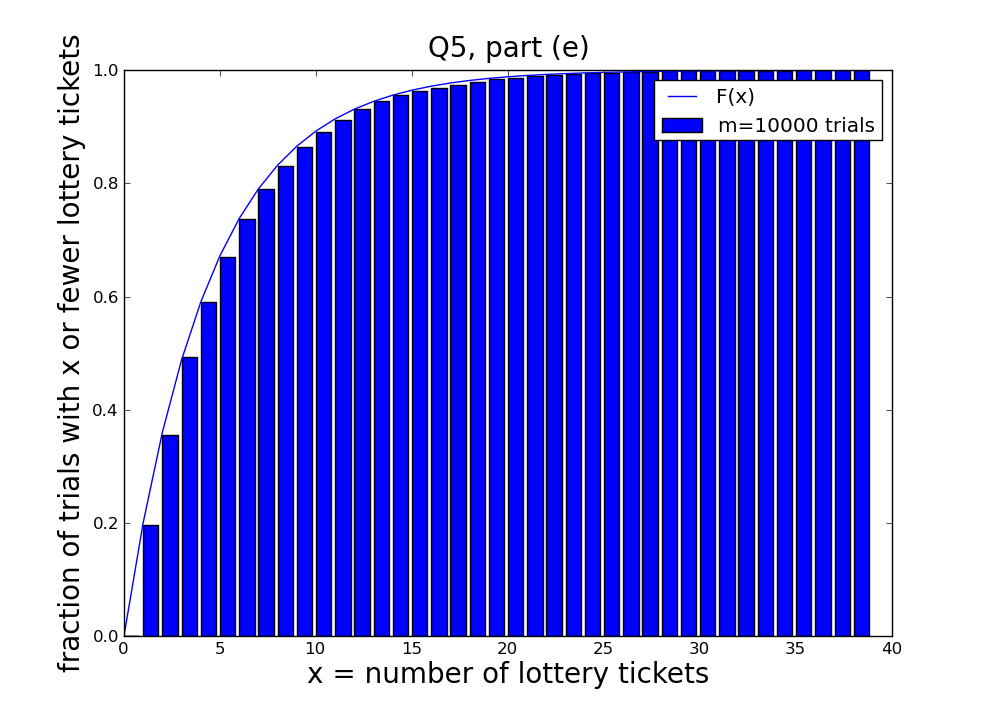
\includegraphics[width=0.95\textwidth]{figures/part_e.png}
\end{figure}
}}\fi


\newpage

\qpart
\item Lastly, we would like to explore a function that defines how many ways you can choose $k$ distinct objects out of $n$ possible objects. This is written as $\binom{n} {k}$ and is read aloud as ``$n$ choose $k$''. We define $\binom{n}{k} = \frac{n!}{k!(n-k)!}$ So, for example, $\binom{5}{3} = \frac{5!}{3!(5-3)!} = \frac{5\cdot 4 \cdot 3 \cdot 2 \cdot 1}{(3 \cdot 2 \cdot 1) \cdot (2 \cdot 1)} = \frac{120}{12} = 10$. We wish to explore this function. Plot the value $\binom{50}{k}$ on the $y$-axis and $k$ on the $x$-axis for $0 \leq k \leq 50$.

Does this constantly grow as $k$ gets larger? What does the shape of the graph remind you of?


\ifsolutions{ \answer { The value of $\binom{n}{k}$ does {\em not} always get larger as $k$ gets larger, it actually peaks around $k=\frac{n}{2}$ and is symmetric around this value. Looking at the plot below, the shape looks very similar to the normal distribution (see part c).

\begin{figure}[h!]
\center
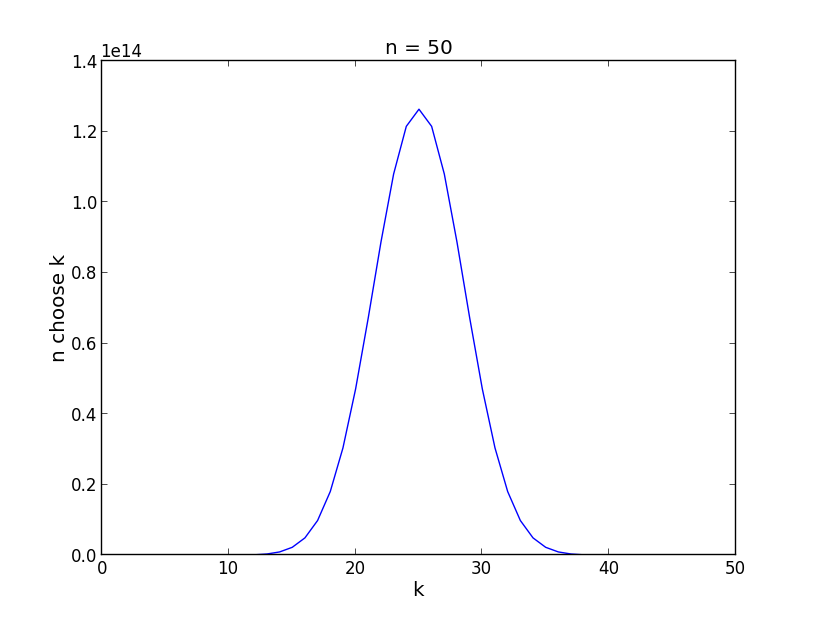
\includegraphics[width=0.6\textwidth]{figures/part_f.png}
\end{figure}
}}\fi

\end{enumerate}

    
\end{qunlist}


\end{document}
